In diesem Kapitel schauen wir uns zuerst an, wie man es aus meiner Sicht eher
\textit{nicht} machen
sollte. Also ein Antipattern der guten Entwicklungspraxis. Leider findet
man solche Code-Schnipsel ohne Warnung auf vielen Tutorial-Seiten. Der Grund
liegt wahrscheinlich darin, dass es sehr einfach und verständlich aussieht.
Und genau darum wollen wir das auch zuerst so machen. Aber keine Sorge - das
Wissen wird nicht vergeblich aufgebaut. Immerhin lernen wir dabei gleich auch
wie SpringBoot funktioniert. So belasten wir uns nicht gleichzeitig mit der
Komplexität des Frameworks und des neuen Ansatzes. Im Laufe des Kapitels
werden wir immer besser und verwandeln unseren anfänglichen Code Schritt für
Schritt in Richtung einer sauberen Architektur. Damit es wirklich ganz einfach
bleibt, wollen wir ein minimales System bauen, um Bücher zu verwalten. Eine
Art Bibliotheksverwaltung aber so simpel wie möglich.

\section{Ganz klassisch: Entity, Controller, Boundary}
ECB (\textit{Entity-Controller-Boundary}) ist eines der klassischen Patterns
das tief in Frameworks wie \textit{Springboot} verankert ist. Es geht 
wahrscheinlich auf das Buch \textit{Object-oriented Software Engineering: 
A Use Case Driven Approach} \cite{jacobson1993} zurück und beschreibt,
wie sich ein Softwaresystem funktional zerlegen lässt. Die Idee dabei
ist einfach. Es gibt eine Modellebene (die \textit{Entities}) in der 
die Datenobjekte modelliert werden, die (Business-)Logik wird in 
\textit{Controllern} separat gehalten und die Darstellung
(oder Präsentation) nach aussen erfolgt über die \textit{Boundary}-Schicht.
In ihrer puren Form hat diese Architektur einige Vorteile. 
\begin{enumerate}
    \item Die Logik bleibt von der Darstellung getrennt
    \item Die Schichten werden über interfaces voneinander
    isoliert. Dabei ist sichergestellt, dass die höheren
    Schichte immer nur auf die unteren Schichten zugreifen
    aber nie umgekehrt.
    \item Zumindest die oberste Schicht ist leicht tausch-
    und erweiterbar, sollte man zukünftig weitere/andere
    Schnittstellen benötigen.
\end{enumerate}

Im Laufe der Jahre wurde dieses Pattern immer wieder abgewandelt und
leider auch geschwächt. Die allseits bekannten \textit{Model-View-Controller}
sind z.B. so ein Negativbeispiel. Dort manipuliert der Controller z.B. direkt
die Präsentation und die Daten.

Beginnend mit \textit{Java-EE} und den \textit{Java Beans} hat sich das ECB
Pattern auch in den Frameworks manifestiert - in leicht abgewandelt und 
erweiterter Form.
\begin{itemize}[resume]
    \item[\textit{Entity}] Die \textit{Entity Beans} repräsentieren Objekte
    aus der Domäne und sind gleichzeitig auch die Datentypen der 
    Persistenz-Schicht. Über \textit{Object-Relational-Mapping} werden diese
    direkt in die Datenbankschicht serialisiert und deserialisiert.
    
    \item[\textit{Controller}] Die Service-Klassen repräsentieren die
    Business-Logik und steuern die Persistenzschicht. Entweder über 
    ausgelagerte Repositories oder direkt über das Framework mittels
    \textit{Entity Manager}. Dabei kommt entweder eine abgewandelte,
    objektorientierte, SQL-Ähnliche Sprache 
    \textit{Java Persistence Query Language} oder natives SQL zum Einsatz.

    \item[\textit{Boundary}] Die Schnittstelle nach aussen wird meist über
    Elemente des Frameworks realisiert um z.B. REST-Endpunkte an die eigene
    Applikation anzubinden. Die Bereitstellung wir dann über einen
    \textit{Applikationsserver} umgesetzt.

\end{itemize}


Bevor wir jetzt anfangen an allem herumzunörgeln, bauen wir das einfach mal
mit Springboot und schauen uns an, was passiert.

Als \textit{Build-Tool} benutzen wir \textit{Maven}, wie im ersten Kapitel
erklärt. Wem die Einführung zu kurz war, der liest am besten noch das Tutorial 
``Maven in 5 Minutes'' \cite{apache2023}. Wer sein Projekt nicht zu Fuss erstellen möchte,
kann gerne auch auf \texttt{https://start.spring.io} für einen Generator
zurückgreifen oder die Funktionen seiner IDE benutzen.
Das entsprechende Repository ist unter den Code-Beispielen unter 
\texttt{bookstack\_trivial}
zu finden. Auf oberster Ebene finden wir neben den Maven-Skripten vor allem 
auch die \textit{pom.xml} - als das zentrale Konfigurationsfile von Maven.
Das wichtigste für uns sind an diesem Punkt die \textit{Dependencies}.
Für unser einfaches Beispiel benötigen wir nur ganz wenige Elemente:

\begin{itemize}
    
    \item\texttt{spring-boot-starter-web}: Die Web-Komponente, damit wir einen
    integrierten Webserver bekommen und unsere REST-Interfaces exponieren
    können.
    \item\texttt{spring-boot-starter-data-jpa}: Der OR-Mapper damit wir eine 
    relationale Datenbank als Backend für unsere Persistenzschicht
    verwenden können.
    \item\texttt{h2}: Eine schlanke SQL In-Memory Datenbank, die man gerne zu
    Entwicklungszwecken benutzt. Man benötigt somit kein anderes DBMS
    und kann später durch Konfigurationsänderung auf Postgres, MariaDB,
    Oracle, oder, oder, oder umsteigen.
    \item\texttt{lombok}: Projekt \textit{lombok} nimmt einen den meisten
    Boilerplate ab, indem es automatisch Getter/Setter/equals/hashcode
    oder toString-Methoden generiert. Auch Konstruktoren muss man
    nicht mehr von Hand schreiben. Funktional notwendig ist das nicht
    aber enorm angenehm.
\end{itemize}

Unser gesamtes Projekt besteht aus gerade mal 5 Source-Files.

\begin{listing}[H]
\begin{minted}{java}
@SpringBootApplication
@AllArgsConstructor
public class BookStack {
        public static void main(String[] args) {
                SpringApplication.run(BookStack.class, args);
        }
}
\end{minted}
\caption{Leere Springboot Main-Klasse}
\label{lst:SpringbootMain}
\end{listing}

Listing \ref{lst:SpringbootMain} reicht bereits komplett aus um unseren
Spring-Kontext zu starten. Da wir \textit{springboot-starter-web} als 
Abhängigkeit eingefügt haben bleibt unsere Applikation am laufen, auch
wenn die Main-Methode beendet wird. Im Hintergrund wird für uns bereits
ein Webserver (\textit{Tomcat} in diesem Fall) gestartet und unsere
Applikation bereits dort automatisch deployed.

\subsection{Persistenz}
Beginnen wir im Stack ganz unten mit der Persistenz. Dazu erstellen wir
eine einfache Java-Klasse mit ein paar Annotationen, wie Listing 
\ref{lst:BookClass} zeigt:

\begin{listing}[H]
\begin{minted}{java}
@Entity
@Data
public class Book {
    @Id
    @GeneratedValue(strategy = GenerationType.IDENTITY)
    public Long id;

    private String title;
    private String isbn;
}
\end{minted}
\caption{Book - Eine Entity-Klasse}
\label{lst:BookClass}
\end{listing}

\texttt{@Entity} ist eine Annotation (technisch eine Art Interface), die
SpringBoot zur Laufzeit auswertet und damit Informationen erhält, was
es mit der Klasse machen soll. \textit{@Entity} bedeutet für Spring
in diesem Fall, dass Instanzen dieses Objekttyps in eine SQL-Tabelle
persistiert werden können. Name der Klasse und ihrer Felder werden
einfach übernommen. Wenn wir das nicht separate konfigurieren 
wird zuerst ein Default-Mapping benutzt 
(\textit{Convention over Configuration}). Wir können alle Namen selbst
bestimmen. Wenn wir aber nichts tun, würden wir eine Tabelle 
\texttt{BOOK} mit den Feldern \texttt{ID, TITLE und ISBN} erwarten.
Mit \texttt{@Id} legen wir den Primärschlüssel fest. Dieser ist somit
automatisch auch unique aud der DB. Die Annotation 
\texttt{@GeneratedValue} legt fest, dass wir Auto-Increment haben möchten.
Fertig! Mehr müssen wir nicht machen.

Damit Spring aber überhaupt weiss, welche Datenbank wir verwenden wollen
müssen wir noch eine Konfigurationsdatei im Projektpfad
\texttt{./src/main/resources/application.properties} anlegen, die
bei uns wie folgt aussieht:

\begin{listing}[H]
\begin{minted}{java}
spring.datasource.url=jdbc:h2:mem:bookstack
spring.datasource.driverClassName=org.h2.Driver
spring.datasource.username=sa
spring.datasource.password=
spring.jpa.hibernate.ddl-auto=update
spring.h2.console.enabled=true
\end{minted}
\caption{Konfiguration über application.properties}
\label{lst:BookClass}
\end{listing}

Wir weisen spring also an die h2 Datenbank in-memory zu
benutzen. Dass wir kein Passwort gesetzt haben ist ok,
wie verwenden das momentan nur lokal. Aber Achtung: 
Die Default-Config würde unsere Anwendung zumindest auf
unserem lokalen Netz nach aussen hin exponieren.

Default-Port ist übrigens 8080, aber auch das wäre in dieser
Datei konfigurierbar.

Mit \texttt{spring.jpa.hibernate.ddl-auto=update} legen
wir zudem fest, dass Spring (in diesem Fall spezifisch 
Hibernate - der verwendete OR-Mapper) uns auch gleich unsere
Tabellen anlegt. \texttt{spring.h2.console.enabled=true}
aktiviert und eine kleine WebApp, mit der wie die Datenbank
verwalten können. Probieren wir das doch mal, indem wir 
unseren Server starten. Das können wir entweder über unsere
Entwicklungsumgebung durch Starten der main-Methode machen
oder auch über das Terminal mittels:

\begin{terminalbox}
    \begin{verbatim}
$ ./mvnw spring-boot:run
    \end{verbatim}
\end{terminalbox}

An dieser Stelle auch gleich ein ``Gesetz'' zum sauberen Aufbau
einer Build-Umgebung:
\begin{rulebox}[label=rule:comandLine]{Ein Java-Projekt ist 
auch über die Kommandozeile erstell- und ausführbar}
Saubere Java-Projekte können über ein Text-Terminal erstellt, gestartet
und getestet werden. Somit bestehen keine spezifischen Abhängigkeiten
zu Entwicklungsumgebungen.
\end{rulebox}

Sollte Spring laufen, können wir uns mit einem Browser auf 
\texttt{http://localhost:8080/h2-console} verbinden und uns einloggen.
Dabei müssen wir darauf achten, dass die DB-URL jenem String aus dem
Konfigurationsfile entspricht. Nutzername: sa, Passwort: <leer>.
Nun können wir unsere Datenbank betrachten (Fig \ref{fig:database}):

\begin{figure}[H]
    \centering
    \includegraphics[width=\textwidth]{./screenshots/BookH2.png}
    \caption{Zustand der Datenbank nach Programmstart}
    \label{fig:database}
\end{figure}

Damit wir auf unsere Objekte in der Datenbank Zugriff bekommen, benötigen
wir noch ein Repository:

\begin{listing}[H]
\begin{minted}{java}
public interface BookRespository extends JpaRepository<Book, Long> {
    Book findByTitle(String title);
    void deleteByTitle(String title);
}
\end{minted}
\caption{Simples Repository für die Book-Entities}
\label{lst:BookRepository}
\end{listing}

Anzumerken ist zu Listing \ref{lst:BookRepository}, dass es sich hierbei
nicht um eine Klasse, sondern nur um ein Interface handelt. Wir werden
das auch gar nicht selber implementieren. Repository-Code ist derart
vorhersehbar, dass Spring uns eine Implementierung zur Laufzeit erzeugt.
Da wir \texttt{JpaRepository} erweitern, bekommen wir schon die ganzen
Standard CRUD-Operaationen wie \texttt{findAll()}, \texttt{findById()}, 
\texttt{delete()} und einige weitere.
Die zusätzlichen Methoden, die wir deklariert haben, folgen einem strikten
Namensmuster. Aus \texttt{findByTitle} wird Spring selbstständig eine
Query a la \texttt{SELECT b FROM Book b WHERE b.title = :title}. Das werden
auch nach der Übersetzung \textit{Prepared SQL Statements} sein, so dass
an diesem Punkt eine SQL-Injection bereits ausgeschlossen wird. Aber das
alles bekommen wir nicht zu Gesicht.

\subsection{Business-Logik}
Natürlich hat die Business-Logik in unserem Trivialbeispiel nicht viel zu 
bieten. Insofern passt die gesamte Klasse auf wenige Zeilen: 

\begin{listing}[H]
\begin{minted}{java}
@Service
public class BookService {
    
    @Autowired
    private BookRespository bookRespository;

    public List<Book> listAllBooks() {
        return bookRespository.findAll();
    }

    public Book createNewBook(String title, String isbn) {
        Book book = new Book();
        book.setTitle(title);
        book.setIsbn(isbn);
        bookRespository.save(book);
        return book;
    }

    public Book bookInfo(String title) {
        return bookRespository.findByTitle(title);
    }

    @Transactional
    public void deleteBook(String title) {
        bookRespository.deleteByTitle(title);
    }

    @Transactional
    public Book updateISBN(String title, String newISBN) {
        Book b = bookRespository.findByTitle(title);
        b.setIsbn(newISBN);
        return b;
    }
}
\end{minted}
\caption{BookService - Implementierung der Business-Logik}
\label{lst:BookService}
\end{listing}

Auch wenn Listing \ref{lst:BookService} trivial scheint, 
hier lohnt es sich, ein paar Details
anzuschauen. Beginnen wir mit \texttt{@Autowired}. Spring bedient sich
eines Patterns, das als \textit{Inversion of Control} \cite{fowler_2004} 
bekannt ist. Kern der Idee ist es nach Möglichkeit nur noch die Interfaces
anzugeben, aber die Instanziierung dem Container zu überlassen. Somit
verschwindet die direkte Abhängigkeit und man könnte zu Testzwecken 
auch eine andere Implementierung einspeisen, sofern sie das Interface
implementiert. Man entkoppelt somit die Schichten.
\texttt{@Service} ist quasi das Gegenteil davon. Damit deklarieren wir 
unsere Klasse gegenüber Spring als Komponenten deren Instanz Spring
verwalten soll und ggf. in ein anderes Objekt (bei uns später) die
Boundary-Schicht injizieren soll. Die letzte Annotation über die wir
noch sprechen müssen ist \texttt{@Transactional}. Wie wir schon
sehen ist die ganze Methode etwas ``magic'' da es so aussieht, als
würden wir gar nicht in die Datenbank schreiben. Und hier kommt der
Trick - Entities, die wir aus der Datenbank bezogen haben sind 
aktiv verwaltet. Sobald wir deren Setter aufrufen, werden die Updates
direkt in die Datenbank geschrieben. Voraussetzung ist dazu, dass wir
uns noch innerhalb einer laufenden Transaktion befinden. Genau 
das haben wir mit der Annotation ausgedrückt. Hat alles geklappt, 
wird am Methodenende ein \textit{Commit} aufgerufen, anderenfalls
folgt ein \textit{Rollback}. Ausserhalb des Transaktionskontexts
werden keine Änderungen meh übernommen.

\subsection{REST-Interface}

Damit sind wir bereits beim \textit{Boundary Layer} angelangt und schauen
uns das REST-Interface an. Genau wie bei den anderen Layern lesen wir 
einfach zuerst den Code:

\begin{listing}[H]
\begin{minted}{java}
@RestController
@RequestMapping("/api/book")
public class BookControllerREST {
    
    @Autowired
    private BookService bookService;

    @GetMapping
    public List<Book> getAllBooks() {
        return bookService.listAllBooks();
    }

    @PutMapping("/{title}")
    public Book updateISBN(@PathVariable String title, @RequestBody String isbn) {
        return bookService.updateISBN(title, isbn);
    }

    @DeleteMapping("/{title}")
    public void deleteBook(@PathVariable String title) {
        bookService.deleteBook(title);
    }

    @PostMapping
    public Book createBook(@RequestBody Book book) {
        return bookService.createNewBook(book.getTitle(), book.getIsbn());
    }
}
\end{minted}
\caption{BookControllerREST.java}
\label{lst:BookControllerREST}
\end{listing}

Auch in diesem Beispiel wird alles über Annotation und Konventionen gesteuert.
\texttt{@RestController} legt fest, dass diese Klasse REST-Antfragen
entgegennehmen kann. mit \texttt{@RequestMapping} wird ein golbaler
Präfix-Pfad festgelegt, die hinteren Pfaddteile werden durch die 
Methodenannotationen vervollständigt. Zur Demonstration habe ich in diesem
Beispiel alle \textit{HTTP-Verben} - also \texttt{GET}, \texttt{PUT},
\texttt{POST} und \texttt{DELETE} verdrahtet. Mit \texttt{@PathVariable}
sehen wir auch schön, wie wir mit dynamischen Pfaden umgehen können.

\subsection{Erste Inbetriebnahme}
Sobald wir unsere Spring-Applikation gestartet haben, können wir das 
Gesamtkonstrukt ``testen''. Testen in Anführungszeichen, da wir hier
mehr um ein herumprobieren sprechen als über wirkliche Tests im Sinne
von Softwaretests. Das machen wir später. Zwar haben wir kein
Frontend aber wir können unser REST-Interface auch einfach mit 
\texttt{curl} ansprechen. Das ist für alle Betriebssysteme verfügbar und
gehört schlicht zur Standardausstattung, wenn man irgendetwas mit dem
HTTP-Protokoll entwickelt. Wer unbedingt möchte, kann auch komplexere
Produkte wie \textit{Postman} einsetzen aber für die ersten Gehversuche
ist das schlicht nicht nötig.

Also probieren wir unseren ersten Request:

\begin{terminalbox}
    \begin{verbatim}
$ curl localhost:8080/api/book 
[]
    \end{verbatim}
\end{terminalbox}

Wie erwartet ist die Antwort die leere Liste - unsere Datenbank ist ja leer.
Einfügen geht aber Problemlos, wir müssen nur einen \textit{POST-Request}
absetzen und ein Buch als \textit{JSON Objekt} im Body mitsenden.

\begin{terminalbox}
    \begin{verbatim}
$ curl \
    -X POST \
    -H "Content-Type: Application/json" \
    -d '{"title":"Hallo, Welt!", "isbn":"123456"}' \
    localhost:8080/api/book

{"id":1,"title":"Hallo, Welt!","isbn":"123456"}
    \end{verbatim}
\end{terminalbox}

Führen wir nun unseren anfänglichen Request nochmals aus, erhalten wir nun
das Buch als einziges Element der Liste zurück:

\begin{terminalbox}
    \begin{verbatim}
$ curl localhost:8080/api/book
[{"id":1,"title":"HalloWelt","isbn":"123456"}]
    \end{verbatim}
\end{terminalbox}

Wenn wir wollen, können wir mit PUT den Titel ändern, auch
wenn das so nicht ganz REST-Konform ist:

\begin{terminalbox}
    \begin{verbatim}
$ curl \
    -X PUT \
    -H "Content-Type: Application/json" \
    -d 'AB12345678' localhost:8080/api/book/HalloWelt
{"id":3,"title":"HalloWelt","isbn":"AB12345678"}
    \end{verbatim}
\end{terminalbox}

Löschen können wir das Buch auch wieder:

\begin{terminalbox}
    \begin{verbatim}
$ curl -X DELETE localhost:8080/api/book/HalloWelt
    \end{verbatim}
\end{terminalbox}

\section{Bewertung des ECB-Patterns}
Eigentlich ist es ja schon erstaunlich, was man in ca. 80 Zeilen Java-Code
alles bekommen kann. Positiv ist sicher die Kürze sowie die Verständlichkeit
unseres Source-Codes. Die Tatsache, dass wir fast alles über Konventionen
statt Konfiguration gelöst haben befreit den Ansatz von fast allem
Boilerplate. Wir haben uns nirgendwo wiederholt (\textit{DRY-Prinzip}) und auch
sonst sind wir fast überall rein fachlich unterwegs gewesen. Selbst der
Boundary-Layer ist auf ein absolutes Minimum beschränkt und reicht die Anfragen
einfach nur gezielt an die Service-Schicht weiter. Also sind wir jetzt fertig
und können so in ein grosses Projekt einsteigen? Na ja ... können vielleicht
schon aber gut ist das aus Architektursicht eigentlich nicht wirklich.

Kein Wunder - bereits Albert Einstein soll ja \textit{``Everything should be 
as simple as possible, but not simpler.''} gesagt haben. Und genau das ist es. 
Es ist zu simpel. Mindestens folgende funktionale Probleme haben wir
erzeugt:

\begin{enumerate}
    \item Keinerlei Input-Validierung. Das heisst ein Buch könnte mit fehlender
    isbn angelegt werden oder schlimmer noch mit fehlendem Titel.
    \item Die ISBN kann ein beliebiger String sein und müsste gar nicht
    dem ISBN-Format entsprechen.
    \item Zwei Bücher könnten mit doppeltem Titel angelegt werden, was dann eine
    eindeutige Abfrage verhindern würde.
    \item Wir leaken Informationen - obwohl es fachlich gar keinen Grund gibt,
    geben wir unsere Datenbank-IDs an die Aussenwelt.
\end{enumerate}

Zudem haben wir auch Architektur-Probleme:

\begin{enumerate}
    \item Nur in der Entity-Schicht wären saubere Unit-Test möglich aber
    in unserem Fall gar nicht relevant, da wir keinerlei prozeduralen
    Code dort erstellt haben.
    \item Bereits die Service-Schicht würde (mehr oder weniger) aufwändige
    Mocks verlangen um isoliert getestet werden zu können. Da wir das
    Repository mit \textit{@Autowired} injecten müsste sogar der ganze
    Spring-Kontext laufen. Das ist dann schon eher ein Integrationstest.
    \item Unser Datenmodell ist Abhängig vom der JPA. Wir sind auf immer
    und ewig an eine relationale Datenbank gebunden. Falls wir das 
    umstellen wollten, müssten wir den ganzen Layer austauschen.
    \item In diesem Trivialbeispiel nicht wirklich sichtbar aber oftmals
    muss man sich nach einer bestehenden Tabellenstruktur richten. Das heisst
    in unser Domänenmodell werden viele Randbedingungen aus der Datenbankwelt
    Einzug erhalten. Obwohl das auf dieser Ebene gar nicht notwendig wäre,
    entwickeln wir so unser Datenmodell entlang der Möglichkeiten relationaler
    Abbildungen. Die Persistenz-Technologie beginnt unser Datenmodell zu
    beeinflussen.
\end{enumerate}

Zumindest die Validierungsprobleme würden sich mit Spring-Bordmittel
adressieren lassen. Wir könnten direkt im REST-Interface
oder auch im Service fordern, dass alle Argumente der Methoden nur
valide Datenelemente wären. Dazu würde man den Methodenparameter mit
\texttt{@Valid} annotieren und die ganze Klasse mit \texttt{@Validated}.
Ebenfalls mit Hilfe von Annotationen würde man das Entity-Modell
anreichern. Für Java ist das in der JSR-380 \cite{jsr380} spezifiziert.
Aber selbst das ist unschön, da wir noch immer durch Programmierfehler
innerhalb unseres Services invalide Objekte erzeugen könnten. Ok, ja
gewisse Kriterien kann man auch nochmals auf der Datenbankschicht
sicherstellen (z.B. \textit{uniqueness} der ISBN). Vielleicht bringt
uns ein ganz anderer Ansatz weiter ...

\section{Immutable Domain Model}
Ohne bereits jetzt zu tief in Paradigmen und Patterns einzutauchen wollen
wir schauen, was wir gewinnen können, wenn wir alles Technische vergessen
und einfach unsere Domäne modellieren. Ohne Abhängigkeiten und ohne
Rücksicht auf irgendetwas. Und wir fordern noch etwas - \textit{immutability}.
Immutable Objects können nicht verändert werden. Sie entstehen durch
Aufruf des Konstruktors und werden (zumindest in Java) durch den
Garbage-Collector beseitigt. Das heisst auch dass alle Validierungen, 
die wir im Konstruktor vornehmen dadurch zu echten \textit{Invarianten}
werden, die immer gelten. Jede Instanz eines Domänenobjekts ist zu 
jedem Zeitpunkt valid. Probieren wir das für unser Bücherverzeichnis.


\begin{listing}[H]
\begin{minted}{java}
public record Book(
        String title,
        String isbn
) {

    public static final Pattern TITLE_PATTERN = Pattern.compile(
            "^[\\p{L}0-9 .,:;!?()'\"-]+$");
    private static final Pattern ISBN_PATTERN = Pattern.compile(
            "^(97(8|9))?\\d{9}(\\d|X)$");

    public Book {
        if (title == null)
            throw new IllegalArgumentException(
                "A book must have a non-null title");
        title = title.trim();
        if (!TITLE_PATTERN.matcher(title).matches())
            throw new IllegalArgumentException("Title has invalid characters.");
        if (title.length() < 4 || title.length() > 60)
            throw new IllegalArgumentException(
                "A book's title must be between 4 and 60 characters");

        if (isbn == null)
            throw new IllegalArgumentException("A book must have a non-null ISBN");
        isbn = isbn.replaceAll("[-\\s]", "").toUpperCase();
        if (!ISBN_PATTERN.matcher(isbn).matches())
            throw new IllegalArgumentException("ISBN has invalid format: " + isbn);
    }
}
\end{minted}
\caption{Book als immutable Domain Object}
\label{lst:BookImmutable}
\end{listing}

Anstelle einer Klasse, nutzen wir im Listing \ref{lst:BookImmutable} 
direkt den Typ \texttt{record}. Damit
bringen wir zum Ausdruck dass wir hier keine Klasse im herkömmlichen
Sinne haben sondern eher ein Value-Object. Sowohl \texttt{title} als auch
\texttt{isbn} sind final, d.h. nur bei der Instanziierung setzbar.
\texttt{public Book {...}} ist der Schluss des Konstruktors. Hier können
wir die Datenfelder auch noch beschreiben und verändern. Und validieren!
Sollte etwas nicht konform sein, werfen wir eine Exception und das Objet
wird gar nicht erst erzeugt. Bei so einem einfachen Datentyp könnte 
man das zwar wirklich so machen aber schöner wäre es die Domäne wirklich
sauber auszumodellieren. Ein Buch hat eben keinen String mit Namen Titel - 
es hat einfach einen Titel. Und eine ISBN. Auch im Normalem Sprachgebrauch
sind das eigentlich eigene Typen. Zerlegt wird das noch stringenter. An 
dieser Stelle zeige ich nur die Titel-Klasse. Die Isbn-Klasse sieht analog
dazu aus und kann im Sourcecode nachgeschaut werden.

\begin{listing}[H]
\begin{minted}{java}
public record Title(
        String text
) {
    
    public static final Pattern PATTERN = Pattern.compile(
        "^[\\p{L}0-9 .,:;!?()'\"-]+$");

    public Title {
        if (text == null)
            throw new IllegalArgumentException("A book must have a non-null title");
        text = text.trim();
        if (!PATTERN.matcher(text).matches())
            throw new DomainValidationException("Title has invalid characters.");
        if (text.length() < 4 || text.length() > 60)
            throw new DomainValidationException(
                    "A book's title must be between 4 and 60 characters");
    }
}
\end{minted}
\caption{Ttiel.java}
\label{lst:TitleClass}
\end{listing}

Mehr Kapselung wie in Listing \ref{lst:TitleClass} ist praktisch nicht zu 
bekommen. Die Funktionalität der Klasse wurde auf ihren minimalen Bereich 
verkleinert. Alles, was man zu einem Buchtitel als Typ sagen kann wird hier 
ausgedrückt. An diesem  Punkt habe ich dem Domain-Model auch noch eine 
einen Exception-Typ \texttt{DomainValidationException} hinzugefügt.
Dieser erbt von  \texttt{RuntimeException} und bringt den Unterschied 
zwischen einem grundsätzlich nichterlaubten Argument 
(wie z.B. \texttt{null}) und einem in dieser Domäne nicht validierbarem
Inhalt zum Ausdruck. Aber das ist nicht unbedingt verpflichtend.

\begin{listing}[H]
\begin{minted}{java}
public record Book(
        Title title,
        Isbn isbn
) {
    public Book {
        if (title == null)
            throw new IllegalArgumentException("A book must have a non-null title");
        if (isbn == null)
            throw new IllegalArgumentException("A book must have a non-null ISBN");
    }
}
\end{minted}
\caption{Book.java}
\label{lst:BookClass}
\end{listing}

Das Buch selbst (Listing \ref{lst:BookClass}) wird damit noch einfacher. 
Es verbleiben nur noch die Null-Checks. Das prüft zwar eine technische
Gegebenheit, ist aber dennoch fachlich motiviert. Eine Instanz von 
\texttt{Book} ist nur dann gültig, wenn sie auch einen
gültigen Titel und eine gültige ISBN besitzt. Jetzt bekommt man schnell
das Gefühl, dass dieser Ansatz sehr viele Klassen erzeugt. Das stimmt aber
das schadet nicht. Ganz im Gegenteil - eine Klasse ist für genau eine
Sache in der Domäne zuständig. Das bringt uns zu einer
weiteren ``Regel'':

\begin{rulebox}[label=rule:numberOfClasses]{Die Qualität einer Codebase
    hängt nicht von der Mange an Klassen ab}
Wir optimieren unsere Codebase nicht nach einer minimalen Anzahl von 
Dateien sondern nach Ausdrucksstärke, Lesbarkeit und Verständlichkeit.
\end{rulebox}

Mit unserem Ansatz gewinnen wir nicht nur Ausdrucksstärke in unseren 
Klassen sondern auch der aufrufende Code wird dadurch transparenter:

\begin{listing}[H]
\begin{minted}{java}
Book book = new Book(
            new Title("Java ist auch eine Insel"),
            new Isbn("978-3-8362-9544-4")
        );
\end{minted}
\caption{Codeschnipsel zur Instanziierung eines \texttt{Book}-Objekts}
\label{lst:createBookSnipped}
\end{listing}

Auch ohne in die Implementierung zu schauen wird an diesem Punkt eindeutig
klar, was die parameter des Konstruktors bedeuten. Das würde sogar jeder
Nicht-programmierer verstehen.

Aber nun kommt der wirkliche Vorteil: Testbarkeit ohne Abhängigkeiten!
\subsection{Domainmodel-Tests}

Was wir an diesem Punkt testen wollen, ist völlig klar - natürlich die
Validierungskriterien. Das sind einfache Unit-Tests auf der Ebene der
einzelnen Typen. 

\begin{listing}[H]
\begin{minted}{java}
class TitleTest {

    @Test
    void rejects_null_title() {
        assertThrows(
                IllegalArgumentException.class,
                () -> new Title(null)
        );
    }

    @Test
    void rejects_too_short_title() {
        assertThrows(
                DomainValidationException.class,
                () -> new Title("DDD")
        );
    }

    @Test
    void rejects_invalid_characters() {
        assertThrows(
                DomainValidationException.class,
                () -> new Title("Clean Code @")
        );
    }
    @Test
    void accepts_invalid_title_with_trim() {
        var title = new Title(" Java ist auch eine Insel ");
        assertEquals("Java ist auch eine Insel", title.text());
    }
}
\end{minted}
\caption{Unit-Test für die Title-Klasse}
\label{lst:createBookSnipped}
\end{listing}

Unser Code hat 4 mögliche Pfade, die wir allesamt testen wollen. Dabei prüfen
wir auch, ob die Exceptions vom richtigen Typ sind und in diesem Fall auch, ob
das Trimmen des Titels wie gewünscht funktioniert.

\begin{rulebox}[label=rule:domainUnitTests]
    {Alle Domain-Objects haben Unit-Tests}
Für alle Domain-Objects entwickeln wir Unit-Tests, die 100\% Path-Coverage für
die Validierung im Konstruktor und etwaiger weiterer Funktionalität aufweisen.
\end{rulebox}

\section{Domain Services}

Dann gibt es noch einen sehr wichtigen Punkt: Wir wollen nicht nur, dass
unser Domänenmodell \textit{immutable} ist - das haben wir bereits erreicht -
sondern dass es ausschliesslich aus \textit{pure functions} besteht. Pure
ist in diesem Fall Synonym für \textit{Seiteneffektfrei}. Jegliche
Funktionen dürfen also nichts am Zustand des Systems verändern. Bei unseren
Domain-Klassen könnten sie das gar nicht (da immutable) aber auch generell
sonst nicht. Damit ist auch sämtlicher I/O verboten, was z.B. Datenbankzugriffe
aber auch selbst Logging einschlisst. Das können wir natürlich nur garantieren,
wenn wir auf diesem Layer geschlossen sind und nur unseren eigenen Code
benutzen. Aufrufe in andere Packages sind damit untersagt - von Java 
Standadfunktionalität mal abgesehen.

\begin{rulebox}[label=rule:pureDomain]
    {Alle Funktionen im Domänenlayer sind Seiteneffektfrei}
Der Domainlayer ist in sich geschlossen. Es bestehen keinerlei Abhängigkeiten
zu anderen (nicht JDK) \textit{Packages}. Alle Funktionen sind frei von
Seiteneffekten und machen - damit einhergehend - keinerlei I/O.
\end{rulebox}

Unsere Domain-Records können neben der Validierung noch weitere Funktionen
haben. Allerdings sollte man darauf achten, dass sich diese Funktionen
nur auf das Domänenobjekt selbst bezieht. Übergeordnete Funktionen sollten
in \textit{Services} ausgelagert werden. Machen wir dazu ein Beispiel, auch
wenn es in diesem einfachen Kontext vielleicht etwas gesucht klingt.
Nehmen wir an, wir möchten fälschlicherweise doppelt erfasste Bücher
identifizieren. Treffen wir dazu die fachliche Entscheidung, dass ein 
Buch dann als doppelt identifiziert wird, wenn es den gleichen Titel
aufweist. Man könnte das wie in Listing \ref{lst:deduplicate} gezeigt 
implementieren:

\begin{listing}[H]
\begin{minted}{java}
public final class DeduplicateBooks {
    public static List<Book> execute(List<Book> inputList) {
        return inputList.stream()
            .collect(Collectors.collectingAndThen(
                    Collectors.toMap(
                        Book::title,
                        Function.identity(),
                        (a, b) -> a,        
                        LinkedHashMap::new),
                    m -> List.copyOf(m.values())));
    }
}
\end{minted}
\caption{Unit-Test für die Title-Klasse}
\label{lst:deduplicate}
\end{listing}

Das mag auf den ersten Blick etwas unkonventionell erscheinen, ist aber
modernes Java. Collectors ind von \texttt{java.util}. Was wir hier
machen ist unsere Liste in eine Map abzubilden, wobei wir den Titel
als Schlüssel und das Book-Objekt direkt als Wert 
(\texttt{Functions.identity()}) für den Eintrag verwenden. Bei doppelten
Einträgen gewinnt immer der Erste \texttt{(a,b)->a}. Am Schluss wird
aus den Werten der (nun duplikatfreien Map) wieder eine Liste erzeugt
und zurückgegeben. Mit \texttt{List.copyOf(...} erzeugen wir uns
übrigens wieder eine immutable List so dass unsere Forderung nach
immutable Objects auch hier erhalten bleibt.

Und natürlich schreiben wir auch hierfür einen kompakten Unit-Test 
(Listing \ref{lst:deduplicateTest}):

\begin{listing}[H]
\begin{minted}{java}
public class DeduplicateBooksTest {

    @Test
    void execute_removesDuplicatesByTitle() {

        Book book1 = new Book(new Title("Clean Code"), new Isbn("978-0-13-235088-4"));
        Book book2 = new Book(new Title("Effective Java"), new Isbn("978-0-13-468599-1"));
        // Duplicate Entry to 1 with modified ISBN
        Book book3 = new Book(new Title("Clean Code"), new Isbn("978-0-13-235088-5"));

        List<Book> input = List.of(book1, book2, book3);

        List<Book> result = DeduplicateBooks.execute(input);

        assertEquals(2, result.size());

        assertEquals(book1, result.get(0));
        assertEquals(book2, result.get(1));
    }
}
\end{minted}
\caption{Unit-Test für den Deduplicate-Service}
\label{lst:deduplicateTest}
\end{listing}

Bis jetzt ist unser Projekt bei folgender Struktur angelangt:


\dirtree{%
.1 srcPackageRoot/.
.2 domain/.
.3 exception/.
.4 DomainValidationException.java/.
.3 model/.
.4 Book.java/.
.4 Isbn.java/.
.4 Title.java/.
.3 service/.
.4 DeduplicateBooks.java/.
.1 testPackageRoot/.
.2 domain/.
.3 model/.
.4 BookTest.java/.
.4 IsbnTest.java/.
.4 TitleTest.java/.
.3 service/.
.4 DeduplicateBooksTest.java/.
}%

Damit ist die Entwicklung unseres Domain-Layers abgeschlossen.

\section{Von Waben und Zwiebeln: Hexagonal- und Onion- Architektur}
Bevor wir weitermachen müssen wir kurz einen Blick auf die Gesamtarchitektur
werfen. Schliesslich wollen wir ja wissen, wo uns die Reise hinführen soll.
Was wir am Schluss bauen wollen folgt der Idee einer 
\textit{Hexagonal Architecture} und darin enthalten auch die Idee der
\textit{Onion Architecture}.

\subsection{Hexagonal Architecture}

Fangen wir bei der hexagonalen Architektur an, dessen Konzept wirklich von 
der ersten Sekunde an überzuegt - leider vom Namen abgesehen. Weder hat das
Ding sechs Seiten noch sechs ecken noch sonst irgendetwas mit Geometrie zu tun.
Dem Internet nach gefiel dem Autor die Form weil es an Waben erinnere. So oder
so, das Pattern geht auf Alistair Cockburn anfangs der 2000er Jahre zurück,
der die \textit{Hexagonal Architecture} in einem gleichnamigen Buch 2024
nochmals beschrieben hat \cite{cockburn_2024}. Im Folgenden werden diese
Ideen verkürzt wiedergegeben.

Der zentrale Punkt des Ansatzes ist die Kapselung eine Stücks zusammenhängender
Business-Logik. In etwa so, wie wir das gerade eben programmiert haben. Mit
Domain-Modell, Domain-Services, Tests - und wie wir gleich sehen werden noch
mit Ports und Adaptern. Die Idee ist auch hier, dass das System innerhalb der
Kapsel (also z.B. innerhalb des Hexagons) nicht von spezifischer Technologie
abhängig ist sondern diese über abstrakte \textit{Ports} einbindet. Das werden
in unserem Fall einfach \textit{Interfaces} sein. Implementiert werden diese
dann über sogenannte \textit{Adapter}, die von aussen an unser Hexagon
``andocken'' und die Funktionalität bereitstellen. Cockburn unterscheidet dabei
zwischen \textit{driving ports} und \textit{driven ports} \cite{cockburn_2024}.
Die einen ``treiben'' unser Hexagon an (also alle Anfragen von aussen), die
Anderen werden von unserem Hexagon aus ``angetrieben'' (z.B. die Datenbank-
Schnittstelle). \textit{Adapters} sind aussen und stellen die technische 
Umsetzung unserer fachlichen Anforderungen der \textit{driven ports} dar.
Oder es sind Komponenten, die uns mit der Aussenwelt verbinden und uns
aufrufen. In Adaptern passiert der gesamte I/O. Dinge wie das REST-Interface,
die Datenbankanbindung Zugriff auf das Dateisystem, das passiert alles 
nur ausserhalb in den Adaptern. Die Implementierung der \textit{driving ports}
(also die direkte Umsetzung der Use-Cases) passiert innerhlb unseres 
Hexagons. Um hier keine Doppeldeutigkeit zu erzeugen nennen wir diese
nicht wie von Cockburn vorgesehen \textit{Interactors} sondern schlicht
\textit{Services}. Cockburn beschreibt 
noch sogenannte \textit{Configurers} die dann die konkreten Implementierungen
an der richtigen Stelle dem System zuführen. Das müssen wir jedoch nicht
implementieren, da uns Springboot genau diese Funktionalität bereits zur
Verfügung stellt.

Bevor das jetzt zu verwirrend wird - einigen wir uns darauf, dass die Ports,
die unser Hexagon treiben nichts anderes als die Sammlung aller 
\textit{Usecases} sind, die wir mit unserer Entwicklung bedienen wollen. An
der Granularität diese Abbildung herrscht allerdings keine Einigkeit. Während 
Cockburn alle Usecases eines Actors zusammenfassen würde und dann quasi
einen Port pro Actor abieten würde, sehen das die Verfechter von
\textit{Clean Architecture} oder \textit{Domain Driven Design} entwas enger
und würden für jeden einzelnen Usecase einen eigenen Port definieren.
Letztlich ist das wohl Geschmacksache - in unserer Umsetzung in Java wäre
das letztlich nur die Frage, ob eine oder mehrere Methoden pro Interface
deklariert werden. Sonst ändert sich nichts. Der Vorteil ist auch hier
Lesbarkeit. Wenn ein Usecase pro Interface definiert ist, und man die
Interfaces halbwegs intelligent benennt, dann sieht man bereits der 
Deklaration der Klasse an, welche Usecases hier bedient werden. Und wieder
ist man der Idee, dass der Code die Dokumentation ist ein Stück näher gekommen.
Wir machen das auch für uns jetzt erst mal so.

Noch eine Randbemerkung zu unserem seiteneffektfreien, immutable und rein 
funktional operierenden Domänenkern. Das kommt übrigens nicht von der
Hexagonal Architecture sondern von einem anderen Pattern: \textit{Functional
Core and Imperative Shell}.

\subsection{Functional Core und Imperative Shell}
Die Idee geht wohl auf einen Vortrag von Gary Bernhardt \cite{bernhardt_2012}
zurück und wurde später in einem Vortrag von Scott Wlaschin reiteriert
\cite{wlaschin_2024}. Beide beschreiben die Idee eines funktionalen Kerns
der (wie wir selbst gesehen haben für exzellente Testbarkeit sorgt) und
nebenbei auch viele Probleme der Threadsicherheit löst. Um damit ein reales
System zu bauen wird erst später (ausserhalb dieses Kerns) I/O erlaubt.
Das ist 1:1 kompatibel mit dem Ansatz der hexagonalen Architektur. I/O
wird dabei sogar ganz nach aussen - also auf ausserhalb des Hxagons verschoben. 

\subsection{Onion Architecture}
Der letzte Architekturbaustein ist die Onion-Architektur. Da muss ich gar
nicht mehr viel dazu sagen, denn diese haben wir bereits vollständig erreicht.
Wit haben bereits eine ganz saubere Schichtentrennung und darüber hinaus
auch eine klare Abhängigkeitshierarchie. Das Domänen-Modell ist unabhängig 
von allem, die Domänen-Services nur von Domänen-Modell. Der Applikationsring
nur von der Domäne. Und alles aussen nur von der Domäne und den Ports.
Es gibt keine einzige Abhängigkeit die in Richtung Aussen zeigen würde.
Und genau das macht den Ansatz so leistungsfähig.

Zusammengefasst bekommt unsere Gesamtarchitektur damit das folgende Bild 
(Abbildung \ref{fig:architecture}). Wie wir sehen, steht unser fachlicher Kern
im Inneren des Hexagons. Dort sind die eben besprochenen \textit{immutable}
Elemente zusammen mit einer technologiefreien Implementierung der 
Usecases. Auf dieser Ebene müssen die Funktionen nicht mehr Seiteneffekt-
aber zumindest technologiefrei sein. Es wird orchestriert aber alles was
nicht zum Domänenkern gehört wird über Interfaces abgetrennt. Das sind die
\textit{Ports}. Erst die technologieabhängigen Adapter implementieren
letztendlich die gesamte I/O-Funktionalität. Somit können die verschiedenen
Architekturansätze, die wir angeschaut haben sinnvoll kombiniert werden.

\begin{figure}[htbp]
  \centering
  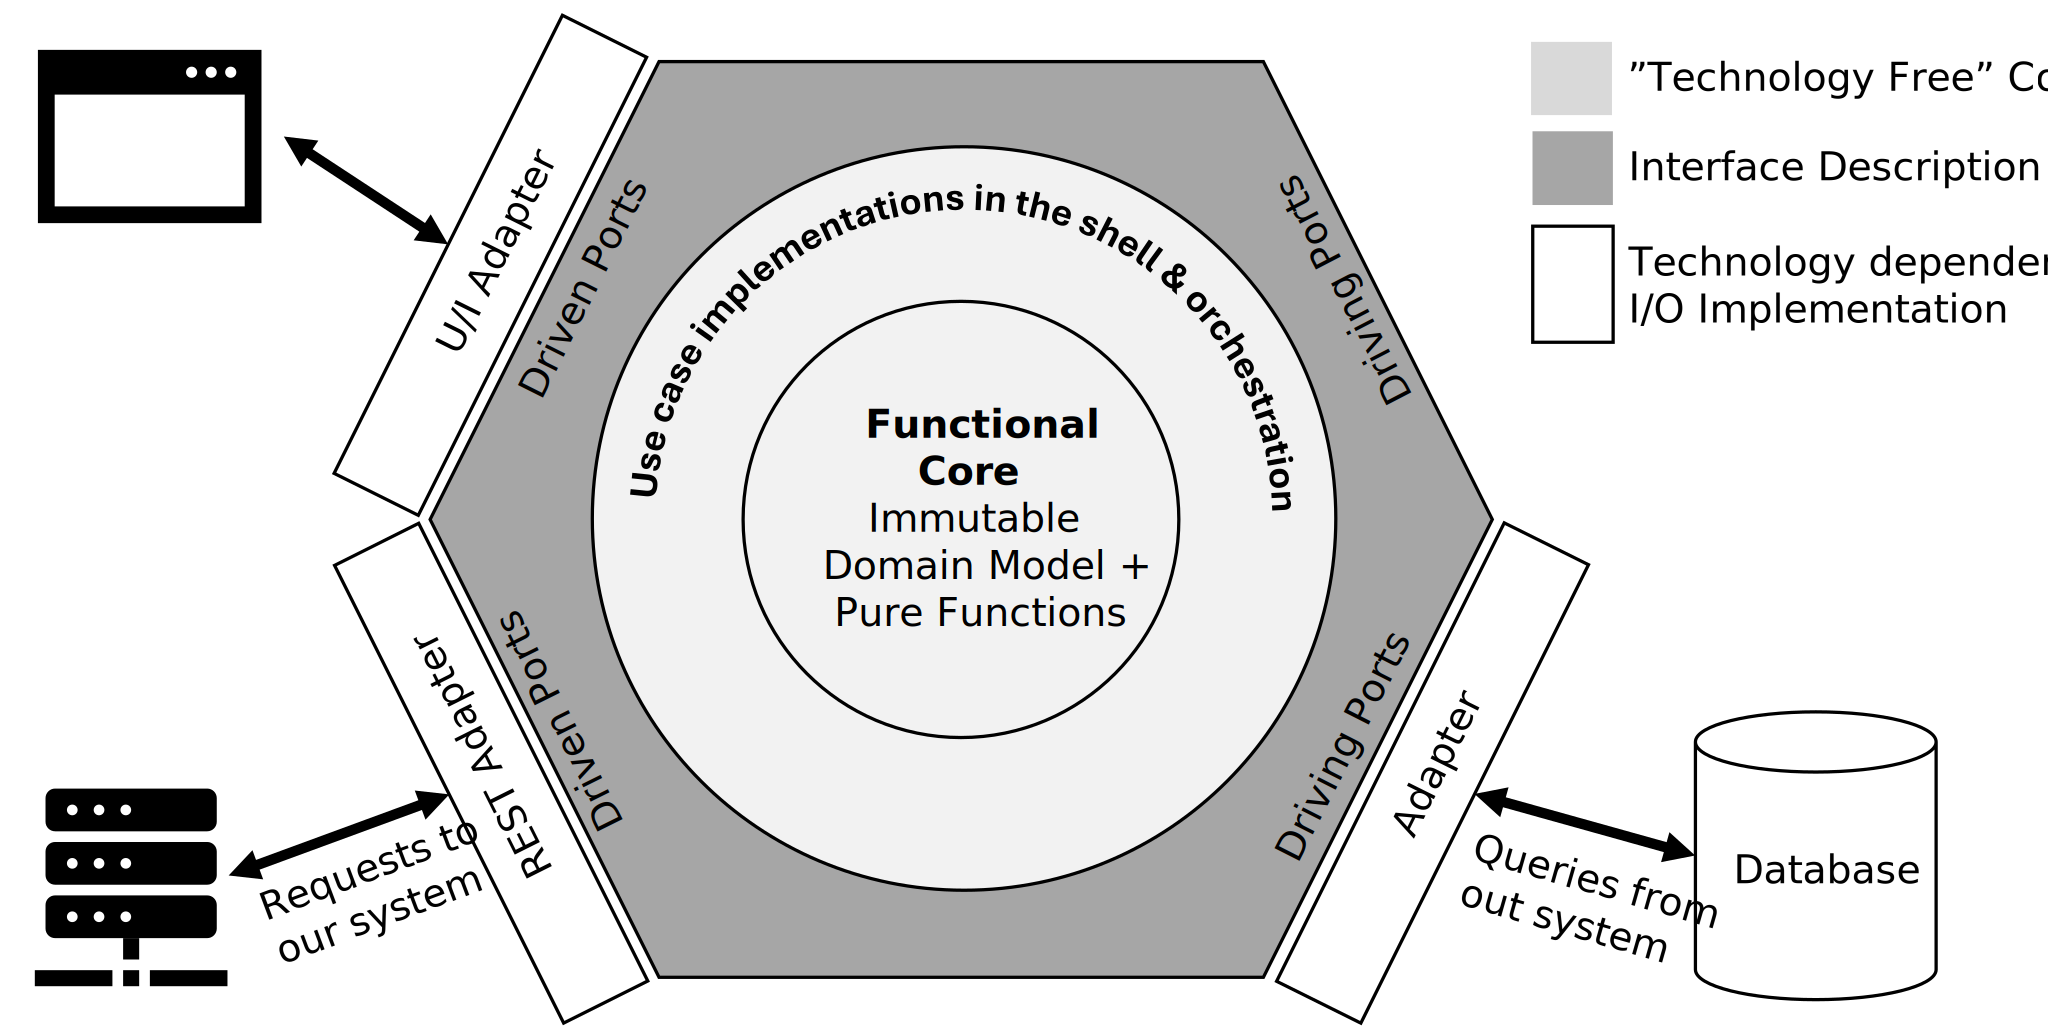
\includegraphics[width=\linewidth]{chapter1/Architecture.pdf}
  \caption{Kombinierte Darstellung der verschiedenen Architekturansätze}
  \label{fig:architecture}
\end{figure}

\section{Die Applikationsschicht}
Am einfachsten verständlich werden diese Architekturkonzepte, wenn man 
sie im Code anwendet. Beginnen wir mit der Definition der Usecases. 
Auch hier ist der Code gleich wieder die Dokumentation. Endlich haben
wir damit auch ein Architekturpattern gefunden in dem sich die Usecases
wirklich auch im Code widerspiegeln. Somit wird die Dokumentation nicht
zur lästigen Pflichtübung sondern ist integraler Bestandteil des Designs,
wie uns Listing \ref{lst:useCases} zeigt:

\begin{listing}[H]
\begin{minted}{java}
public interface ListAllBooksUseCase {
    List<Book> listAllBooks();
}

public interface LookupBookUseCase {
    Optional<Book> lookupIsbn(Isbn isbn);
}

public interface RegisterBookUseCase {
    void register(Book book);
}
\end{minted}
\caption{Die drei UseCases der Applikation}
\label{lst:useCases}
\end{listing}

Usecases sind in diesem Fall einfache Interfaces, die selbsterklärende
Namen haben sollten. Alleine im Verzeichnisbaum kann man so bereits
grob sehen, was die Applikation tut, sprich welche Usecases im Design
vorgesehen wurden.

Zu Demonstrationszwecken implementieren wir diese Usecases in zwei
Service-Klassen. Man hätte auch alles in eine einzige Klasse packen können
aber ich wollte an diesem Punkt die Gestaltungsfreiheit zeigen.

\begin{listing}[H]
\begin{minted}{java}
@Service
public class QueryBooksService implements ListAllBooksUseCase, LookupBookUseCase {

    private final BookPersistence findBook;

    public QueryBooksService(BookPersistence findBook) {
        this.findBook = findBook;
    }

    @Override
    public List<Book> listAllBooks() {
        return findBook.findAll();
    }

    @Override
    public Optional<Book> lookupIsbn(Isbn isbn) {
        return findBook.findBy(isbn);
    }
    
}
\end{minted}
\caption{Implementierung der ListAll- und Lookup Usecases}
\label{lst:lookupUseCase}
\end{listing}

Zugegeben, listing \ref{lst:lookupUseCase} sieht leer und redundant aus. 
Die Anfragen werden einfach durchgereicht. Das liegt aber mehr an der 
Trivialität unserer Applikation als an der Architektur. Aber ist das nicht
grossartig, wie sich die erste Zeile bereits liest? Da steht ja fast in 
lesbarem Englisch "Die Klasse QueryBooksService implementiert die beiden
Usecases ListAllBooks und LookupBook". Mehr müssen wir gar nicht wissen.

Was wir noch nicht besprochen haben ist, wo die BookPersistence auf einmal
herkommt. Hier kommen die \textit{driving ports} oder \textit{out ports} ins
Spiel. Da wir uns noch innerhalb unseres Hexagons befinden dürfen wir uns 
noch nicht auf eine spezielle Implementierung festlegen - insofern ist das
ebenfalls ein Interface (Listing \ref{lst:bookPersistence}).

\begin{listing}[H]
\begin{minted}{java}
public interface BookPersistence {
    List<Book> findAll();
    Optional<Book> findBy(Isbn isbn);
    void save(Book book);
}
\end{minted}
\caption{BookPersistence outbound Port}
\label{lst:bookPersistence}
\end{listing}

Die Zweite Service-Klasse ist übrigens zumindest etwas interessanter, da
sie fachliche Logik widerspiegelt (Listing \ref{lst:RegisterBookService}).
An dieser Stelle haben wir festgelegt, dass ein Buch nicht persistiert werden
darf, fall ein anderes Buch bereits mit dieser ISBN registriert ist.

\begin{listing}[H]
\begin{minted}{java}
@Service
public final class RegisterBookService implements RegisterBookUseCase {

    private final BookPersistence bookPersistence;

    public RegisterBookService(
            BookPersistence bookPersistence
    ) {
        this.bookPersistence = bookPersistence;
    }

    @Override
    public void register(Book book) {
        if (bookPersistence.findBy(book.isbn()).isPresent()) {
            throw new IllegalStateException(
                "Book with ISBN " + book.isbn().value() + " already exists"
            );
        }
        bookPersistence.save(book);
    }
}
\end{minted}
\caption{Implementierung des RegisterBook Usecase}
\label{lst:RegisterBookService}
\end{listing}

Man beachte das \textit{@Sercive} über der Klasse. Das wäre eigentlich von der
Architektur her verboten, denn es stellt eine technische Abhängigkeit der
Klasse zu Spring her. Wenn man das sinnvoll argumentieren kann, dann lohnt
sich zuweilen ein gewisser Pragmatismus. So auch in diesem Fall. 
\textit{@Sercive}\ ändert nichts am Verhalten der Komponente und könnte bei der
Portierung einfach gelöscht werden. Bei den Tests haben wir alleine schon 
wegen den späteren Integrations- und Systemtests die Abhängigkeiten zu Spring
auf Projektebene(!) ohnehin. Insofern ändert sich rein gar nichts und wir 
ersparen uns dabei das redundante erstellen von den \textit{Configurers}.
Spring beherrscht Dependency-Injection bereits in nahezu Perfektion.

\subsection{Applikationsschicht - Tests}
Testen ist auch auf der Applikationsschicht notwendig und sinnvoll. Aufgrund
unserer sauberen Architektur können wit aber selbst auf dieser Ebene noch
vollständig auf UnitTests zurückgreifen. Vor allem haben wir an dieser Stelle
beinahe perfekt vorbereitete ``Units'' - es sind unsere Usecases! Das eignet
sich gut, denn das sind ja genau abgegrenzte \textit{units of work}.

Es reicht an dieser Stelle nur einen der Tests zu zeigen, die anderen beiden
funktionieren völlig analog zu Listing \ref{lst:RegisterBookUseCaseTest}.

\begin{listing}[H]
\begin{minted}{java}
public class RegisterBookUseCaseTest {
    
    private static BookPersistence bookPersistence;
    private static RegisterBookUseCase usecase;

    @BeforeEach
    void setup() {
        bookPersistence = new InMemoryBookPersistenceAdapter();
        usecase = new RegisterBookService(bookPersistence);
    }

    @Test
    void registers_book_if_not_existing() {
        var book = new Book(
                new Title("Domain-Driven Design"),
                new Isbn("9780321125217")
        );
        usecase.register(book);
        assertTrue(bookPersistence.findBy(book.isbn()).isPresent());
    }

    @Test
    void rejects_book_with_existing_isbn() {
        var book = new Book(
                new Title("Domain-Driven Design"),
                new Isbn("9780321125217")
        );
        usecase.register(book);
        assertThrows(
                IllegalStateException.class,
                () -> usecase.register(book)
        );
    }
}
\end{minted}
\caption{RegisterBookUseCase Unit Test}
\label{lst:RegisterBookUseCaseTest}
\end{listing}

Damit der Test laufen kann benötigen wir ein funktionierendes Repsoitory.
Man hätte die echte Datenbank nehmen können - aber dann würde es wieder 
zu einem Integrationstest. Allerdings ist unsere Persistenzschicht derart
einfach, dass man sich einfach eine In-Memory-Implementierung schreiben kann:

\begin{listing}[H]
\begin{minted}{java}
public final class InMemoryBookPersistenceAdapter
        implements BookPersistence {

    private final Map<Isbn, Book> store = new HashMap<>();

    @Override
    public Optional<Book> findBy(Isbn isbn) {
        return Optional.ofNullable(store.get(isbn));
    }

    @Override
    public void save(Book book) {
        store.put(book.isbn(), book);
    }

    @Override
    public List<Book> findAll() {
        return store.values().stream().toList();
    }
}

\end{minted}
\caption{InMemoryBookPersistenceAdapter}
\label{lst:InMemoryBookPersistenceAdapter}
\end{listing}

Mehr als in Listing \ref{lst:InMemoryBookPersistenceAdapter} braucht es gar 
nicht, damit wir testen können. 
Somit sind wir fertig und fügen dem Projekt auf dieser Schicht folgende
Files hinzu:

\dirtree{%
.1 srcPackageRoot/.
.2 application/.
.3 port/.
.4 in/.
.5 ListAllBooksUseCase.java/.
.5 LookupBookUseCase.java/.
.5 RegisterBookUseCase.java/.
.4 out/.
.5 BookPersistence.java/.
.3 service/.
.4 QueryBooksService.java/.
.4 RegisterBookService.java/.
.1 testPackageRoot/.
.2 adapters/out/memory/.
.3 InMemoryBookPersistenceAdapter.java/.
.2 application/.
.3 ListAllBooksUseCase.java/.
.3 LookupBookUseCase.java/.
.3 RegisterBookUseCase.java/.
}%

Somit ist unser Applikationskern fertig. Mit 25 Java-Files und 685 Zeilen 
Code haben wir einen sehr sauberen Applikationskern erstellt, dessen 3 
Usecases mit 16 Tests überprüft wurden. Das ist natürlich ein grosser Schritt
von den 137 Zeilen des trivialen Codes, der zudem noch die ganze REST- und 
Persistenzanbindung enthielt. Das ist jedoch genau der Preis, den man in Bezug
auf architektonische Excellenz und sauberen Tests bezahlt. Anzahl von Zeilen
Code waren eben noch nie ein guter Prädiktor für die Qualität oder der 
Verständlichkeit einer Software. Aber nun wollen wir den Rest der Applikation
noch vervollständigen.

\section{Adapters}
Im Wesentlichen benötigen wir zwei Adapter, die an unsere Ports andocken.
Einmal den REST-Adapter, der die Schnittstelle nach aussen exponiert und
einemal unseren Pesistenzadapter, der die Anbindung an die Datenbank
implementiert.

\subsection{Persistence Adapter mit JPA}

Der Auftrag ist klar - wir müssen lediglich das Interface BookPersitance aus 
Listing \ref{lst:bookPersistence} implementieren. Das werden wir ziemlich 
Analog zu dem Code aus dem trivialen Beispiel umsetzen.

\begin{listing}[H]
\begin{minted}{java}
@Entity
@Data
@AllArgsConstructor
public class BookEntity {
    @Id
    private String isbn;
    private String title;
}
\end{minted}
\caption{BookEntity mit voller JPA und Lombok-Annotation}
\label{lst:BookEntity}
\end{listing}

In Listing \ref{lst:BookEntity} wird die ISBN direkt als Primärschlüssel
verwendet. Ob das performance-technisch eine gute Idee ist, kommt
darauf an, ob es noch andere Relationen gibt, die auf diesen
Primärschlüssel verweisen. Anderenfalls sollte man doch auf eine
nummerische ID ausweichen.

Um effektiv darauf zugreifen zu können, bneötigen wir noch das passende
Repository (Listing \ref{lst:BookRepository}) was in diesem
Fall leer ist, da wir mit der Standard-Funktionalität auskommen.

\begin{listing}[H]
\begin{minted}{java}
public interface BookRepository extends 
    JpaRepository<BookEntity, String> {
    
}
\end{minted}
\caption{Leeres BookRepository nur mit JPARepository Standardfunktionen}
\label{lst:BookRepository}
\end{listing}

Somit haben wir bereits alle Teile beisammen um den Adapter zu
finalisieren. Es fehlt nur noch seine eigentlich Implementierung,
wie in Listing \ref{lst:JpaBookPersistenceAdapter} gezeigt:

\begin{listing}[H]
\begin{minted}{java}
@Service
public class JpaBookPersistenceAdapter
        implements BookPersistence {

    private final BookRepository bookRepository;

    public JpaBookPersistenceAdapter(BookRepository bookRepository) {
        this.bookRepository = bookRepository;
    }

    @Override
    public Optional<Book> findBy(Isbn isbn) {
        return bookRepository.findById(isbn.value())
                .map(this::toDomain);
    }

    @Override
    public List<Book> findAll() {
        return bookRepository.findAll()
            .stream()
            .map(this::toDomain)
            .toList();
    }

    @Override
    public void save(Book book) {
        bookRepository.save(fromDomain(book));
    }

    private Book toDomain(BookEntity entity) {
        return new Book(
                new Title(entity.getTitle()),
                new Isbn(entity.getIsbn())
        );
    }

    private BookEntity fromDomain(Book book) {
        return new BookEntity(
                book.isbn().value(),
                book.title().text()
        );
    }
}
\end{minted}
\caption{Der JPA Persistenz-Adapter}
\label{lst:JpaBookPersistenceAdapter}
\end{listing}

Nichts davon solle wirklich überraschend sein ausser die beiden privaten
Funktionen \texttt{fromDomain} und \texttt{toDomain}. Da unsere
Entity-Klasse sehr einfach aufgebaut ist und lediglich Strings
benutzt müssen wir zwischen diesen beiden Repräsentationen umwandeln.
Hier sei angemerkt, dass die Umwandlung \texttt{toDomain} bereits
die volle Validierung vornimmt. Wir erinnern uns - ein invalides
Domänenobjekt ist nicht intanziierbar. In gegenrichtung können wir
uns darauf verlassen, dass wir keine invaliden Objekte an die 
Datenbank liefern, da bereits das Interface an die Persistenz
nur über Domänenobjekte definiert wurde. Somit können wir an dieser
Stelle auf weitere Checks verzichten und sind fertig.

Noch ein letzter Hinweis: Persistence ist nur ein Beispiel einer
Service-übergreifender I/O Funktionalität. Logging würde man identisch
mittels eines Ports und eines Adapters implementieren.

\subsection{REST Adapter mit Springboot-web}

Um das Ganze an die Aussenwelt anzubinden müssen wir eine Komponente 
(einen \textit{Adapter}) schreiben, der unsere \textit{driven ports}
entsprechend ansteuert.

\begin{listing}[H]
\begin{minted}{java}
@RestController
@RequestMapping("/api/books")
public class BookController {
    
    private final RegisterBookUseCase registerBookUseCase;
    private final ListAllBooksUseCase listAllBooksUseCase;
    private final LookupBookUseCase lookupBookUseCase;
    
    BookController(
            RegisterBookUseCase registerBook,
            ListAllBooksUseCase listAllBooksUseCase,
            LookupBookUseCase lookupBookUseCase) {
        this.registerBookUseCase = registerBook;
        this.listAllBooksUseCase = listAllBooksUseCase;
        this.lookupBookUseCase = lookupBookUseCase;
    }
    ...
    @GetMapping("/{isbn}")
    ResponseEntity<BookDto> getBook(@PathVariable String isbn) {
        return ResponseEntity.of(
                lookupBookUseCase.lookupIsbn(new Isbn(isbn))
                        .map(this::fromDomain));
    }
    ...
    private BookDto fromDomain(Book book) {
        return new BookDto(
                book.title().text(),
                book.isbn().value());
        }
}
\end{minted}
\caption{REST-Adapter implementiert in BookController.java}
\label{lst:BookController}
\end{listing}

Auch in Listing \ref{lst:BookController} ist die Verwendung der Usecases
erneut sehr schön zu sehen und im Wortlaut zu verstehen. Dieser Controller
steuert die Usecases \textit{RegisterBook}, \textit{ListAllBooks} und
\textit{LookupBook} an. Perfekt - wir wissen sofort um was es geht. An 
dieser Aussenschnittstelle endet auch unsere Domäne. Es wäre ein Zufall,
wenn unsere Aussenwelt die Formate unsere Domäne so 1:1 verwenden könnte.
Daher setzen wir \textit{Data-Transfer-Objects} - oder kurz \textit{DTOs}
ein um den Datenaustausch nach aussen zu beschreiben. Da unser Beispiel
inhaltlich trivial ist, gibt es hier wirklich ein 1:1-Mapping, ausser bei den
Datentypen. Wir bekommen Strings und lifern ein BookDTO 
(Listing \ref{lst:BookDTO}) als record mit Strings
für die Felder. Bei komplexeren Anforderungen ist es auch üblich nach
RequestDTOs und ResponseDTOs zu unterscheiden. So wie es halt von den
Anforderungen her nötig ist. Das Mapping mittels \texttt{fromDomain}
und \texttt{toDomain} kennen wir bereits aus dem Persistenz-Adapter.

\begin{listing}[H]
\begin{minted}{java}
public record BookDto (
        String title,
        String isbn
) {
}
\end{minted}
\caption{BookDTO.java}
\label{lst:BookDTO}
\end{listing}


Zudem legen wir noch eine Konfigurationsklasse an, damit Spring die Exceptions
aus unserem Domain-Model richtig behandelt. In diesem Fall wollen wir nicht
\texttt{500 Internal Server Error} zurückgeben sondern lieber 
\texttt{400 Bad Request} und den Text der Exception als Content zurückliefern.
Ob man so transparent sein möchte ist vor allem eine Securityentscheidung.
Wir machen das einfach mal.

\begin{listing}[H]
\begin{minted}{java}
@ControllerAdvice
public class RestExceptionHandler {

    @ExceptionHandler({
        IllegalArgumentException.class,  
        DomainValidationException.class})
    public ResponseEntity<String> handleBadRequestExceptions(RuntimeException ex) {
        return ResponseEntity
                .status(HttpStatus.BAD_REQUEST)
                .body(ex.getMessage());
    }
}
\end{minted}
\caption{Konfiguration um Exceptions richtig zu behandeln}
\label{lst:RestExceptionHandler}
\end{listing}

\subsection{Adaptertests als Integrationstests}
Damit bleibt nur noch unsere Adapter zu testen. Ob man an dieser Stelle
Unittest benötigt hängt von der Komplexität der Adapter ab. Für unsere
Zwecke genügen an dieser Stelle Integrationstests, da wir eigentlich nur
fachlich langweiliges I/O in diesen Adaptern realisieren. Den Applikationskern
und die Domäne haben wir ja bereits ausführlich getestet.

\begin{listing}[H]
\begin{minted}{java}
@SpringBootTest
@Transactional
public class JpaBookPersistenceAdapterTest {
    
    @Autowired
    JpaBookPersistenceAdapter adapter;

    @Test
    void persists_and_loads_book() {
        Book book = new Book(
                new Title("Effective Java"),
                new Isbn("9780134685991")
        );

        adapter.save(book);
        assertTrue(adapter.findBy(book.isbn()).isPresent());
    }
}
\end{minted}
\caption{Integrationtest des JpaBookPersistenceAdapter}
\label{lst:JpaBookPersistenceAdapterTest}
\end{listing}

Listing \ref{lst:JpaBookPersistenceAdapterTest} zeigt wie einfach wir einen
Integrationstest bewerkstelligen können. Mit \texttt{@SpringBootTest} und
\texttt{@Transactional} starten wir den Springboot-Context und sorgen
dafür dass unsere Testdaten nicht final in die Datenbank geschrieben werden.
Es erfolgt ein \textit{Rollback} am Ende der Testmethode.
Das wäre bei unserer In-Memory-H2-Datenbank zwar unwichtig aber es ist am 
saubersten das gleich so zu spezifizieren.

Final testen wir nun noch unseren REST-Adapter (Listing \ref{}).

\begin{listing}[H]
\begin{minted}{java}
@SpringBootTest
@AutoConfigureMockMvc
@ActiveProfiles("inmemorytest")
@Transactional
class BookControllerTest {

    @Autowired
    MockMvc mockMvc;

    @Autowired
    BookRepository bookRepository;

    @Test
    void registerAndLoadBook() throws Exception {
        mockMvc.perform(post("/api/books")
                .contentType(MediaType.APPLICATION_JSON)
                .content("""
                            {
                              "title": "Effective Java",
                              "isbn": "9780134685991"
                            }
                        """))
                .andExpect(status().isOk());

        mockMvc.perform(get("/api/books"))
                .andExpect(status().isOk())
                .andExpect(jsonPath("$.length()").value(1));

        mockMvc.perform(get("/api/books/9780134685991"))
                .andExpect(status().isOk())
                .andExpect(jsonPath("$.title")
                        .value("Effective Java"));
    }

    @Test
    void testExceptionHandling() throws Exception {
        mockMvc.perform(post("/api/books")
            .contentType(MediaType.APPLICATION_JSON)
            .content("""
                        {
                            "title": "",
                            "isbn": "9780134685991"
                        }
                    """))
            .andExpect(status().is4xxClientError());
    }
}
\end{minted}
\caption{Integrationstest des REST Controllers}
\label{lst:BookControllerTest}
\end{listing}

Damit ist aus Sicht der Entwicklungs- und Testarbeit am Backend alles getan.
In der Aussenschicht um unser Hexagon herum haben wir folgende Dateien dem 
Projekt hinzugefügt:

\dirtree{%
.1 srcPackageRoot/.
.2 adapters/.
.3 in/.
.4 rest/.
.5 BookController.java/.
.5 BookDto.java/.
.5 RestExceptionHandler.java/.
.3 out/.
.4 persistance/.
.5 BookEntity.java/.
.5 BookRepository.java/.
.5 JpaBookPersistenceAdapter.java/.
.1 testPackageRoot/.
.2 adapters/.
.3 in/.
.4 rest/.
.5 BookControllerTest.java/.
.3 out/.
.4 persistence/.
.5 JpaBookPersistenceAdapterTest.java/.
}%

Damit ist das Backend final fertig. Mit 808 Zeilen Code und total 19 
Tests haben wir eine saubere, zukunftssichere sehr verständliche 
Architektur umgesetzt.

\section{Diskussion des Ansatzes}
Natürlich muss man das immer relativieren. Der Ansatz ist für sehr kleine
Projekte sicher ein ``overkill'' und selbst bei grösseren Unterfangen nicht
immer notwendig. Wenn man sich sehr sicher ist, dass der verwendete
Technologiestack sich nicht mehr ändert (also dass man z.B. von 
Springboot und einer relationalen Datenbank nicht abweicht) kann man auch
bewusst eine Abhängigkeit in Kauf nehmen. Ebenso, was den funktionalen Kern
angeht. Es ist eine (zugegeben extrem saubere) Möglichkeit eine 
Domäne in Code abzubilden. Aber wir wissen ja aus unzähligen Projekten davor,
dass es noch viele weitere gute Möglichkeiten gibt dies zu tun. 
Die Lösung, die wir hier angeschaut haben bringt klar mehr Komplexität. Das ist
erst mal schlecht - es kommt jedoch darauf an, welche Form von Komplexität man 
anhäuft (\textit{incidental} vs. \textit{accidental} \textit{complexity}).
Gegen \textit{incidental complexity} kann man nicht viel machen - die passiert
einfach, oder liegt einfach vor. Wenn die modellierte Domäne komplex ist, wird
das automatisch auch komplexeren Code nach sich ziehen (oder zumindest mehr 
Code). Wer jetzt denkt, dass
das Domänenmodell in unserem naiven Code den Sachverhalt viel weniger Komplex 
abbilden konnte, der irrt insofern, als dass das Modell es verpasst hat die 
Komplexität überhaupt abzubilden. Im Endeffekt ist das noch schlimmer - 
erforderliche Komplexität die in Code und Tests ignoriert wird. Das ist 
natürlich ein Problem denn so entsteht fehlerhafte Software. Durch fehlende
Validierung und ein Modell, dass inkonsistente und falsche Repräsentationen
erlaubt entstehen auch schnell echte Sicherheitsprobleme. So oder so, die
Domäne muss schon adäquat abgebildet werden.
Anders sieht es bei der Zwiebel-, hexagonalen oder Ports und Adapter- 
Architektur aus. Je nach Betrachtungsweise ist diese Zerlegung und Abstraktion
genau nicht von der Domäne vorgegeben und motiviert. Das ist allein unsere
Entscheidung, die wir aus Gründen der Testbarkeit, wiederverwendbarkeit, 
Flexibilität der Technologie oder einfach nur zur Aufteilung der Bereiche in
in grossen Teams treffen. Passiert das unüberlegt, dann baut man 
\textit{accidential complexity} auf. Unnötig Komplexität anzuhäufen ist so wie
sonst im Leben Risiken einzugehen ohne einen Ertrag zu erwarten - Eine
dumme Entscheidung!

Um dafür ein besseres Gespür zu erhalten wollen wir eine deutlich
komplexere Domäne Modellieren und ein ganzes System mit Frontend sowie 
technischer Anbindung erstellen um diesen Entscheidungsraum etwas besser 
zu erforschen.